\documentclass[conference]{IEEEtran}
\usepackage{hyperref}
\IEEEoverridecommandlockouts
% The preceding line is only needed to identify funding in the first footnote. If that is unneeded, please comment it out.
\usepackage{cite}
\usepackage{amsmath,amssymb,amsfonts}
\usepackage{algorithmic}
\usepackage{graphicx}
\usepackage{textcomp}
\usepackage{xcolor}
\def\BibTeX{{\rm B\kern-.05em{\sc i\kern-.025em b}\kern-.08em
    T\kern-.1667em\lower.7ex\hbox{E}\kern-.125emX}}
\begin{document}

\title{Bearing Fault Diagnosis Based on Signal Processing\\
\thanks{Homework of the course ICE4405P-Digital Signal Processing}
}

\author{\IEEEauthorblockN{1\textsuperscript{st} Nan Lin}
\IEEEauthorblockA{\textit{Shanghai Jiao Tong University} \\
\textit{Shanghai, China} \\
lns\_brandon@sjtu.edu.cn}
\and
\IEEEauthorblockN{2\textsuperscript{nd} Yanxu Meng}
\IEEEauthorblockA{\textit{Shanghai Jiao Tong University} \\
\textit{Shanghai, China}\\
meng-mou-xu@sjtu.edu.cn}
}

\maketitle

\begin{abstract}
Bearing fault diagnosis is critical for predictive maintenance and reliability in rotating machinery. This paper presents an advanced approach using signal processing techniques, specifically Kurtogram and Envelope Analysis, to detect and analyze fault-induced vibrations in bearings. The Fast Kurtogram identifies optimal frequency bands where fault signatures are prominent, while Envelope Analysis demodulates signals to reveal characteristic fault frequencies. The analysis, conducted using Python, demonstrates how these techniques accurately identify fault types and locations in faulty bearings. Results show enhanced accuracy and timeliness of fault detection, supporting proactive maintenance strategies and improving operational reliability. The project's code is available on GitHub for further research and application.
\end{abstract}

\begin{IEEEkeywords}
Bearing Fault Diagnosis, Signal Processing, Kurtogram, Envelope Analysis, Predictive Maintenance, Vibration Analysis, Fast Fourier Transform (FFT), Python.
\end{IEEEkeywords}

\section{Introduction}

Bearing fault diagnosis is a critical aspect of predictive maintenance and reliability engineering in rotating machinery. Bearings are fundamental components in many industrial applications, and their failure can lead to significant operational disruptions and economic losses. Therefore, early detection and accurate diagnosis of bearing faults are essential to prevent unexpected breakdowns and extend the lifespan of machinery.

This paper presents an advanced approach to bearing fault diagnosis based on signal processing techniques. The methodology involves the use of Kurtogram and Envelope Analysis, which are powerful tools for detecting and analyzing fault-induced vibrations in bearings. The Fast Kurtogram provides an efficient way to identify the optimal frequency bands where bearing fault signatures are most prominent. Envelope Analysis, on the other hand, is employed to demodulate the vibration signals, making it easier to detect characteristic fault frequencies.

The signals are processed to extract features that indicate the presence and severity of faults such as inner race, outer race, and rolling element defects. The analysis is conducted using Python, which offers robust capabilities for signal processing and visualization.

Through a detailed examination of the vibration signals, the paper demonstrates how the combination of Kurtogram and Envelope Analysis can effectively diagnose bearing faults. The results show that these techniques can accurately identify fault types and their locations, providing valuable insights for maintenance planning and machinery health management.

In summary, this paper contributes to the field of condition monitoring by offering a reliable and efficient method for bearing fault diagnosis. The proposed approach enhances the accuracy and timeliness of fault detection, thereby supporting proactive maintenance strategies and improving the operational reliability of industrial machinery.

The code related to this project could be found in the \href{https://github.com/Languisher/DSP-Project-202405}{GitHub repository}.

\section{Background}

\subsection{Random Signal Processing}

The Random Signal Processing Method is utilized to analyze the stochastic properties of vibration signals generated by bearings. This method involves several key steps, including signal acquisition, preprocessing, and statistical analysis.

We suppose that the reader has already mastered the essence of this undergraduate course.

\subsection{Resonance Modulation Method}

When local damage occurs on the working surface of a bearing, repeated impacts between the bearing and other contacting components generate concentrated impact pulses. Due to their extremely short duration and wide frequency range, these impact pulses induce high-frequency resonance in the equipment, thereby amplifying the fault pulses.

Steps in the Resonance Demodulation Method:
\begin{enumerate}
    \item \textbf{Detection of High-Frequency Resonance Pulses}: The impact pulses caused by local damage are typically high-frequency signals. When analyzing bearing faults through spectrum analysis, it is often difficult to identify low-frequency information within these high-frequency signals.
    \item \textbf{Band-Pass Filtering and Envelope Analysis}: To isolate the high-frequency vibration signals, band-pass filtering is employed. The specific frequency band for filtering is determined through kurtosis analysis, which identifies the frequency range where the resonance pulses are most pronounced. A band-pass filter with a specific center frequency and bandwidth is then used to extract the frequency band of interest.
    \item \textbf{Amplitude Demodulation to Form the Envelope Signal}: After band-pass filtering, amplitude demodulation is performed to generate an envelope signal. By observing the spectrum of the envelope signal, it becomes possible to identify the characteristic frequencies associated with bearing faults at lower frequencies. This process allows for a more intuitive judgment and identification of faults.
\end{enumerate}

\section{Theory}
\subsection{Envelope Extraction}\label{env}

First, we extract the envelope of the vibration signal. The envelope extraction is performed using the Hilbert transform, which is a common technique in signal processing to obtain the analytic signal. The envelope is then computed as the magnitude of the analytic signal.

The mathematical formulation for the Hilbert transform and the envelope extraction is as follows:

\subsubsection{Hilbert Transform}
\begin{equation}
\hat{x}(t) = \mathcal{H}\{x(t)\} = \frac{1}{\pi} \text{P.V.} \int_{-\infty}^{\infty} \frac{x(\tau)}{t - \tau} d\tau
\end{equation}
where \(\mathcal{H}\{x(t)\}\) is the Hilbert transform of \(x(t)\), and P.V. denotes the Cauchy principal value.

\subsubsection{Analytic Signal}
\begin{equation}
z(t) = x(t) + j\hat{x}(t)
\end{equation}
where \(z(t)\) is the analytic signal.

\subsubsection{Envelope}
\begin{equation}
\text{Envelope}(t) = |z(t)| = \sqrt{x(t)^2 + \hat{x}(t)^2}
\end{equation}

\subsection{Frequency Domain Analysis}

Next, we perform a frequency domain analysis on the envelope signal using the Fast Fourier Transform (FFT). This helps in identifying the characteristic fault frequencies.

The mathematical formulation for the FFT and power spectrum computation is as follows:

\subsubsection{Fast Fourier Transform (FFT)}
\begin{equation}
X(f) = \sum_{n=0}^{N-1} x(n) e^{-j2\pi fn/N}
\end{equation}
where \(X(f)\) is the FFT of \(x(n)\), and \(N\) is the number of samples.

\subsubsection{Frequency Bins}
\begin{equation}
f_k = \frac{k}{N \Delta t}
\end{equation}
where \(f_k\) is the frequency corresponding to the \(k\)-th bin, and \(\Delta t\) is the sampling interval.

\subsubsection{Power Spectrum}
\begin{equation}
P(f) = |X(f)|^2
\end{equation}

\subsection{Spectral Kurtosis Analysis}\label{spekur}

The spectral kurtosis analysis is a powerful technique used to identify non-Gaussian components in a signal, which are often indicative of faults in machinery. In this analysis, the spectral kurtosis is computed and visualized to highlight frequencies and time windows where the signal exhibits impulsive behavior. The following explains the theoretical background and the practical implementation of the spectral kurtosis analysis based on the provided code.

Spectral kurtosis is a statistical measure that quantifies the "peakedness" or impulsiveness of a signal within a specific frequency band. It is particularly useful in fault diagnosis because fault-induced signals typically exhibit higher kurtosis values compared to normal operational signals. Kurtosis is used to measure the "tailedness" or impulsiveness of the filtered signal, which helps in identifying fault characteristics. A high kurtosis value indicates the presence of significant impulsive components. The kurtosis of the filtered signal \( x(t) \) is given by:

\subsection{Bandpass Filter}

After we have calculated the necessary "tailedness" or impulsiveness of the signal, we then perform the signal to a Bandpass filter. Bandpass filtering is a signal processing technique used to isolate a specific range of frequencies from a broader signal. It allows frequencies within a certain range (band) to pass through while attenuating frequencies outside this range. The Butterworth filter is commonly used for this purpose due to its flat frequency response in the passband.

The filter design involves defining the low and high cutoff frequencies and the filter order. The cutoff frequencies are normalized by the Nyquist frequency. Mathematically, the bandpass filter design can be expressed as:

\begin{equation}
\text{low} = \frac{\text{lowcut}}{\text{nyq}}, \quad \text{high} = \frac{\text{highcut}}{\text{nyq}}
\end{equation}

where \(\text{nyq} = 0.5 \times \text{fs}\) is the Nyquist frequency, and \(\text{fs}\) is the sampling frequency. The Butterworth filter coefficients are calculated using:

\begin{equation}
b, a = \text{butter}(\text{order}, [\text{low}, \text{high}], \text{'bandpass'})
\end{equation}

The filtered signal \( y \) is obtained by applying the filter to the data:

\begin{equation}
y = \text{lfilter}(b, a, \text{data})
\end{equation}

\section{Experiment}

\subsection{Observation of the Signals}

We take the signal in 100.csv file as an example. First, we plot the time-domain representation of the signal, which is displayed in Figure \ref{fig_1}. Next, we perform a Fast Fourier Transform (FFT) on the signal, and the resulting frequency-domain representation is shown in Figure \ref{fig_2}.

\begin{figure}[htbp]
    \centerline{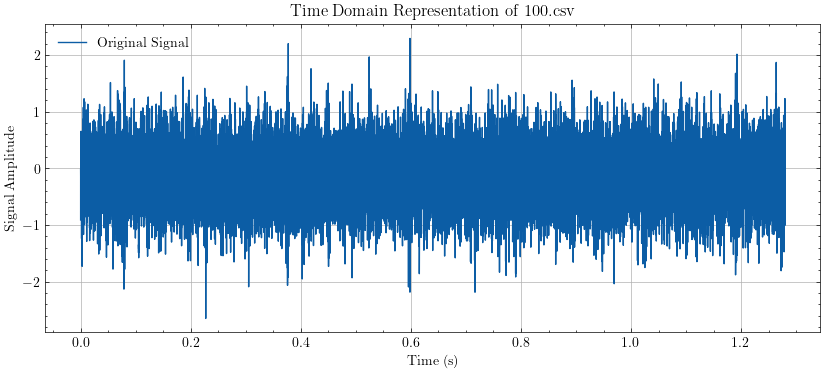
\includegraphics[width=0.5\textwidth]{figure/fig_1.png}}
    \caption{Time Domain Representation of 100.csv}
    \label{fig_1}
\end{figure}

\begin{figure}[htbp]
    \centerline{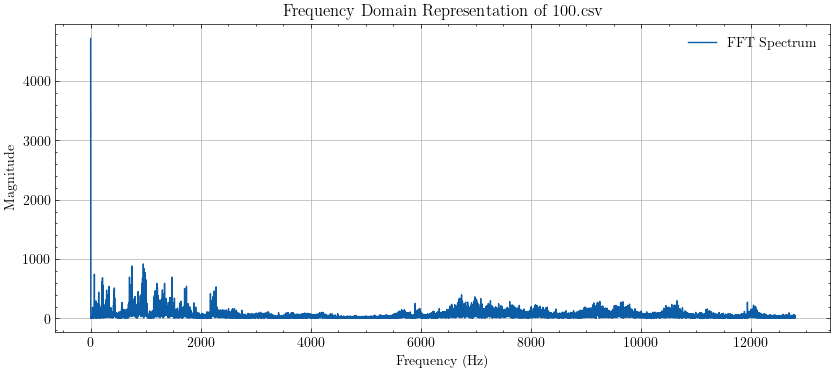
\includegraphics[width=0.5\textwidth]{figure/fig_2.png}}
    \caption{Frequency Domain Representation of 100.csv}
    \label{fig_2}
\end{figure}

\subsection{Envelope Spectrum}

Using the theory discussed in Section \ref{env}, we plot the time-domain representation of the enveloped signal of 144.csv in Figure \ref{fig_3}.

\begin{figure}[htbp]
    \centerline{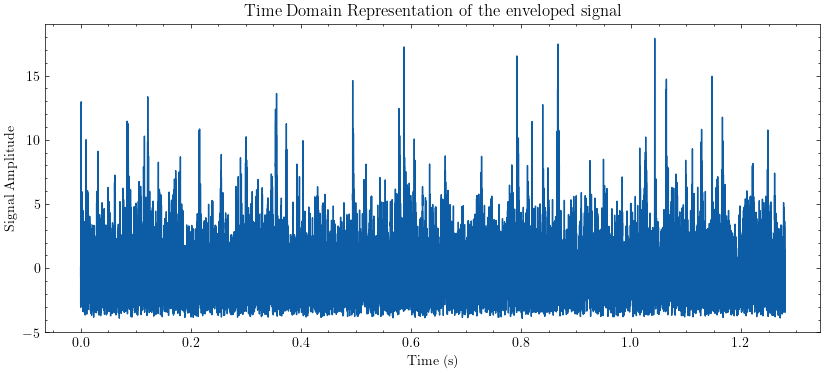
\includegraphics[width=0.5\textwidth]{figure/fig_3.png}}
    \caption{Time Domain Representation of the enveloped signal of 144.csv}
    \label{fig_3}
\end{figure}

Then we perform a FFT on the signal, and the resulting frequency-domain representation is shown in Figure \ref{fig_4}.

\begin{figure}[htbp]
    \centerline{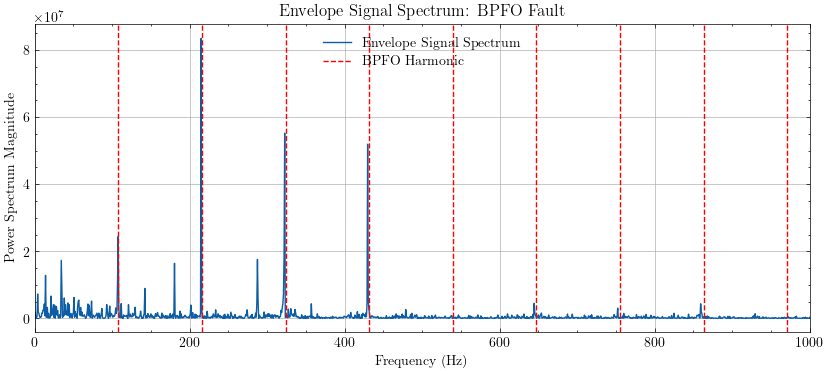
\includegraphics[width=0.5\textwidth]{figure/fig_4.png}}
    \caption{Frequency Domain Representation of the enveloped signal of 144.csv. It could be seen that the envelope signal spectrum corresponds neatly with the BPFO Harmonic, which demonstrates that its fault characteristic is BPFO}
    \label{fig_4}
\end{figure}

\subsection{Kurtogram Analysis}

Using the theory discussed in Section \ref{spekur}, the Kurtogram of the signal 144.csv is displayed in Figure \ref{fig_5}.

\begin{figure*}[htbp]
    \centerline{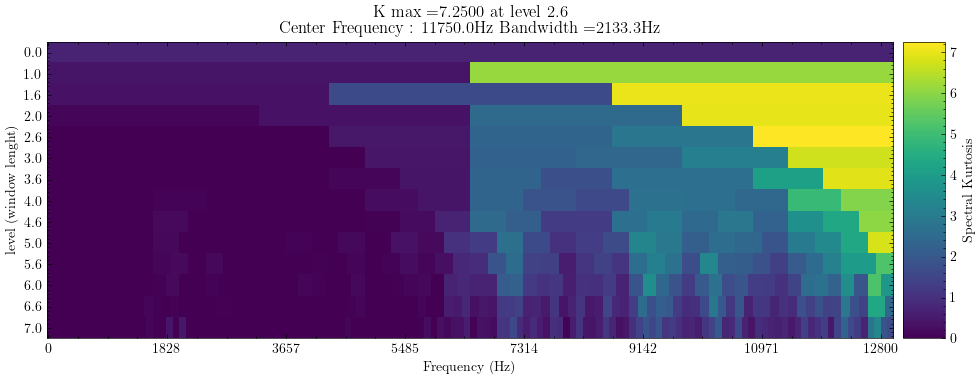
\includegraphics[width=\textwidth]{figure/fig_5.png}}
    \caption{Kurtogram of 144.csv. We could observe that the frequency is centered at 11750.0Hz with a bandwidth of 2133.3Hz}
    \label{fig_5}
\end{figure*}

With the calculated results, we then perform the signal to a bandpass filter. Here, we design the low cutoff frequency and high cutoff frequency the center frequency plus (minus resp.) a third of the bandwidth.

The result is in Figure \ref{fig_6}.

\begin{figure*}[htbp]
    \centerline{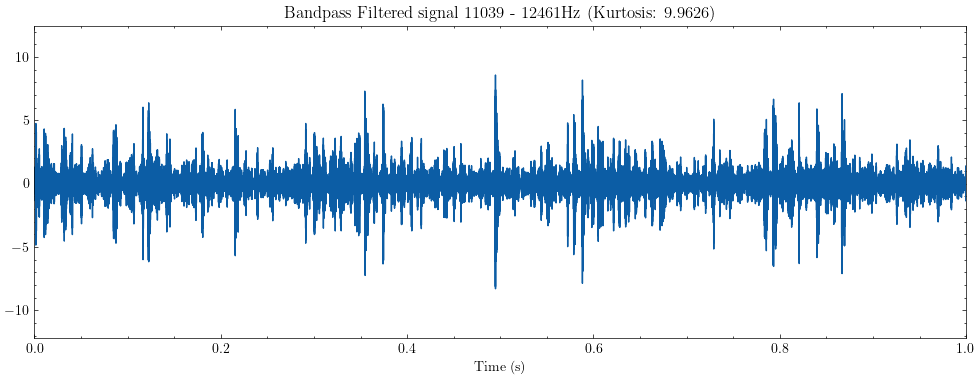
\includegraphics[width=\textwidth]{figure/fig_6.png}}
    \caption{Time Domain Representation of the filtered signal of 144.csv}
    \label{fig_6}
\end{figure*}

Finally, we obtain the result after performing an FFT to the signal once more, which demonstrates that the signal displays the fault characteristic of BPFO.

\begin{figure*}[htbp]
    \centerline{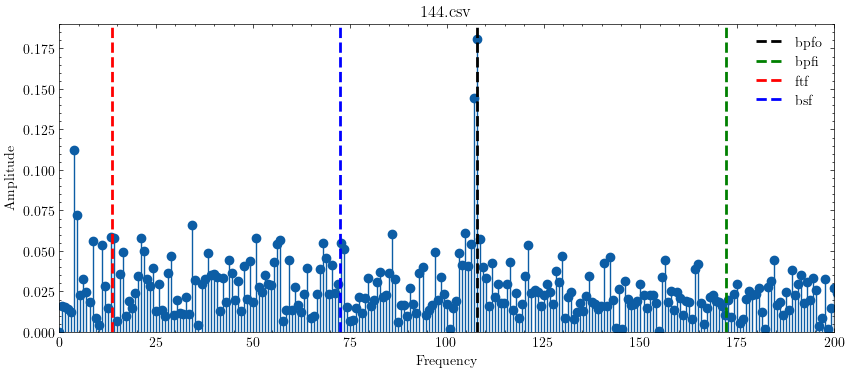
\includegraphics[width=\textwidth]{figure/fig_7.png}}
    \caption{Frequency Domain Representation of the filtered signal of 144.csv}
    \label{fig_7}
\end{figure*}

\subsection{Result}

The result of all the signals is shown in Figures \ref{fig_11} to \ref{fig_15}. From the results, we can conclude the fault characteristics as shown in Table \ref{result}:

\begin{table}[htbp]
\caption{Failure Modes of 8 Faulty Samples}
\begin{tabular}{lllllll}
Data Files & $n$ & $fr(rps)$ & $d(mm)$ & $D(mm)$ & $A$ & Failure Mode \\
100.csv    & 8   & 35        & 7.92    & 34.55   & 0   & FTF \& BPFO  \\
110.csv    & 8   & 35        & 7.92    & 34.55   & 0   & BPFO         \\
123.csv    & 8   & 35        & 7.92    & 34.55   & 0   & BPFO         \\
144.csv    & 8   & 35        & 7.92    & 34.55   & 0   & BPFO         \\
161.csv    & 8   & 37.5      & 7.92    & 34.55   & 0   & BPFO         \\
486.csv    & 8   & 37.5      & 7.92    & 34.55   & 0   & BPFO         \\
2365.csv   & 8   & 40        & 7.92    & 34.55   & 0   & BSF \& BPFO  \\
2538.csv   & 8   & 40        & 7.92    & 34.55   & 0   & BPFO        
\end{tabular}
\label{result}
\end{table}

\begin{figure*}[htbp]
    \centerline{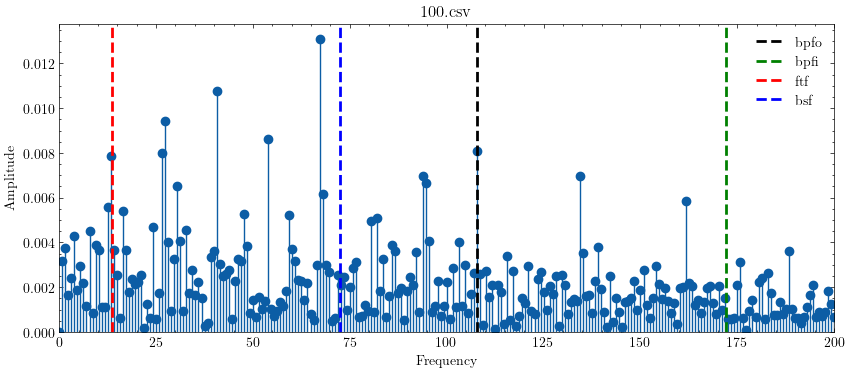
\includegraphics[width=\textwidth]{figure/fig_11.png}}
    \caption{Fault Diagnosis Analysis of Signal 100.csv}
    \label{fig_11}
\end{figure*}

\begin{figure*}[htbp]
    \centerline{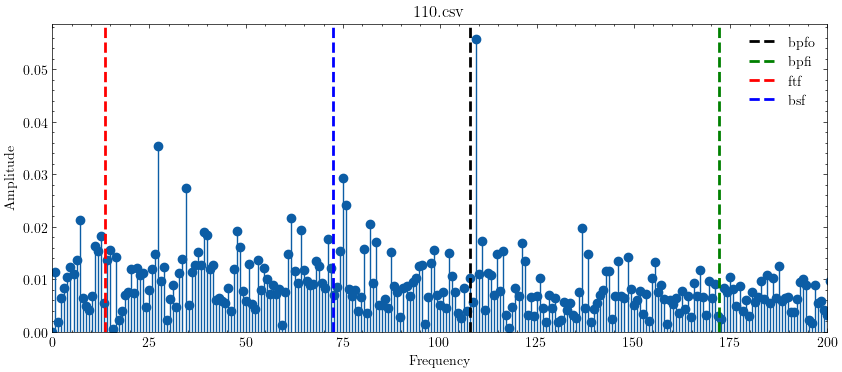
\includegraphics[width=\textwidth]{figure/fig_13.png}}
    \caption{Fault Diagnosis Analysis of Signal 110.csv}
    \label{fig_13}
\end{figure*}

\begin{figure*}[htbp]
    \centerline{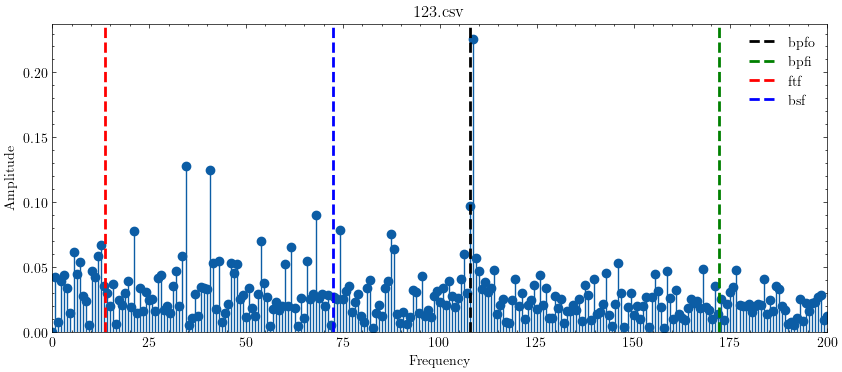
\includegraphics[width=\textwidth]{figure/fig_10.png}}
    \caption{Fault Diagnosis Analysis of Signal 123.csv}
    \label{fig_10}
\end{figure*}

\begin{figure*}[htbp]
    \centerline{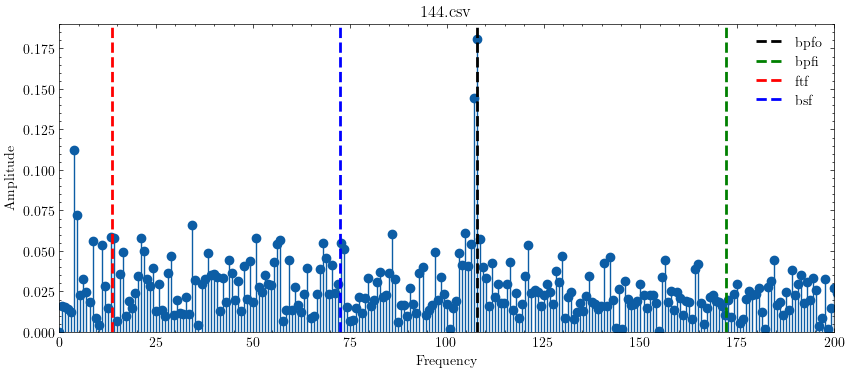
\includegraphics[width=\textwidth]{figure/fig_8.png}}
    \caption{Fault Diagnosis Analysis of Signal 144.csv}
    \label{fig_8}
\end{figure*}

\begin{figure*}[htbp]
    \centerline{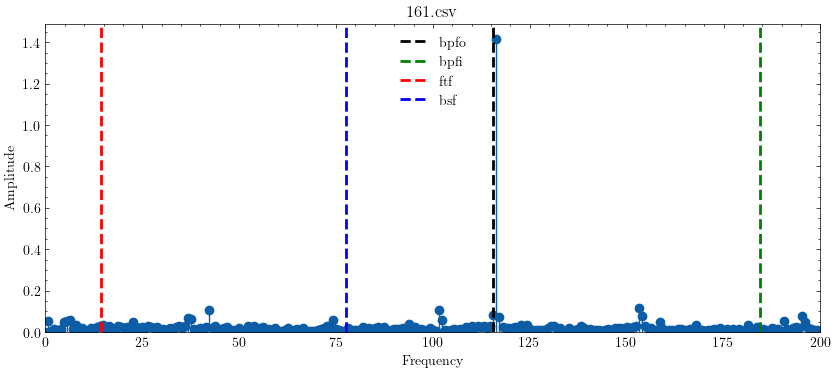
\includegraphics[width=\textwidth]{figure/fig_14.png}}
    \caption{Fault Diagnosis Analysis of Signal 161.csv}
    \label{fig_14}
\end{figure*}

\begin{figure*}[htbp]
    \centerline{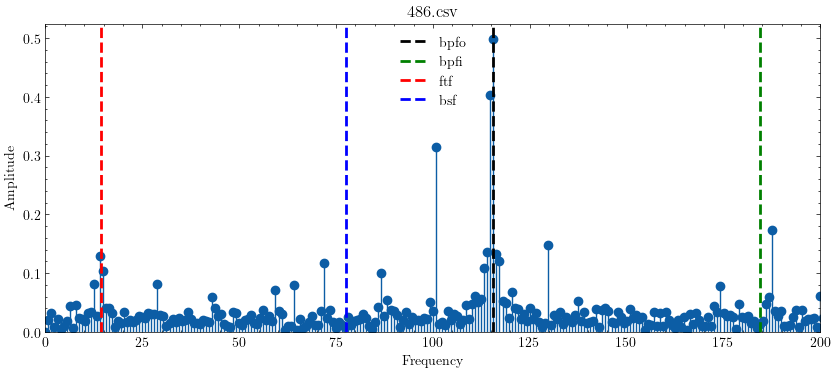
\includegraphics[width=\textwidth]{figure/fig_9.png}}
    \caption{Fault Diagnosis Analysis of Signal 486.csv}
    \label{fig_9}
\end{figure*}

\begin{figure*}[htbp]
    \centerline{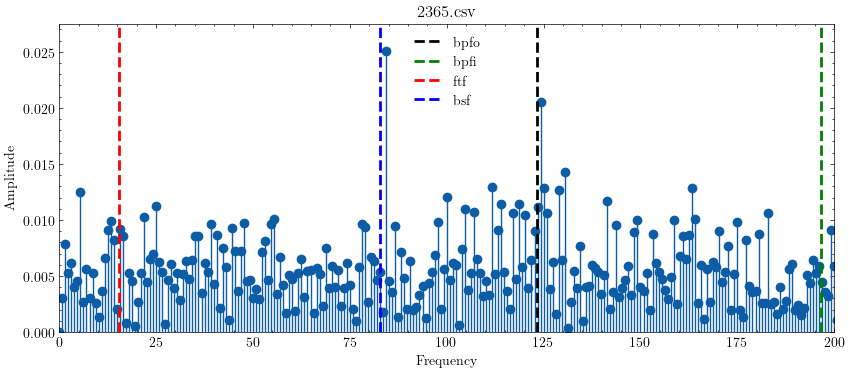
\includegraphics[width=\textwidth]{figure/fig_12.png}}
    \caption{Fault Diagnosis Analysis of Signal 2365.csv}
    \label{fig_12}
\end{figure*}

\begin{figure*}[htbp]
    \centerline{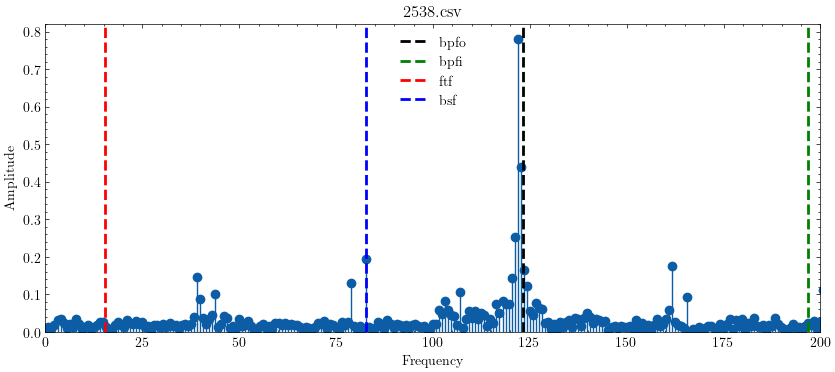
\includegraphics[width=\textwidth]{figure/fig_15.png}}
    \caption{Fault Diagnosis Analysis of Signal 2538.csv}
    \label{fig_15}
\end{figure*}

\end{document}
